% !TEX TS-program = pdflatex
% !TeX encoding = UTF-8
% !TeX spellcheck = en_GB
%=======================================================================
%== Template for LaTeX presentation ====================================
%=======================================================================
\providecommand{\PathP}{./parts/} 		% Path to Parts folders
\providecommand{\PathR}{./resources/} 	% Path to Resources folders
\providecommand{\PathSO}{./sources/} 	% Path to Sources folders
\providecommand{\PathS}{./supplies/} 	% Path to Supplies folders
\providecommand{\BuildTrigger}{buildnew} % Trigger to build or not standalone parts.
\providecommand{\langue}{english}		% english, french

\makeatletter
	\def\input@path{{\PathSO}{\PathSO/gotham}{\PathSO/Inria/}} 		% to be able to find package in resource folders.
	\ifx\c@levelstanda\undefined 	% to create a newcounter if it doesn't exists.
		\newcounter{levelstanda}
	\else
		{}% it already exist
	\fi
\makeatother


\documentclass[notheorems, noamsthm, aspectratio=169, 10pt]{beamer}
	% use this instead for 16:9 aspect ratio: [aspectratio=169]
	% supported aspect ratios  1610  169 149 54 43 (default) 32
	%
	% The option "handout, " allows to the print the hidden slides made by <handout:1|beamer:0>[noframenumbering].
	%
	% the option "notes=only, " to print only the notes !
	\usepackage[l2tabu, orthodox]{nag}	% Help to prevent buggus with warnings

%-=-=-=-=-=-=-=-=-=-=-=-=-=-=-=-=-=-=-=-=-=-=-=-=
%        DEFAULT PACKAGES
%-=-=-=-=-=-=-=-=-=-=-=-=-=-=-=-=-=-=-=-=-=-=-=-=
	\usepackage[utf8]{inputenc}
	\usepackage[T1]{fontenc}


%-=-=-=-=-=-=-=-=-=-=-=-=-=-=-=-=-=-=-=-=-=-=-=-=
%        BEAMER OPTIONS
%-=-=-=-=-=-=-=-=-=-=-=-=-=-=-=-=-=-=-=-=-=-=-=-=
	% Gotham Theme
	\usetheme{gotham}
	\usetheme{gothamInria}
		\InriaSet{RF}% {RF,old1,old2,old3}
	% \usetheme{gothamCEA}
	% 	\CEASet{official}% {official}

		% Apply all Gotham setting.
		\gothamset{
			% format frametitle=titlecase,
			% format title=titlecase, format section=titlecase,
			% sectionframe default=on, sectiontocframe default=on,
			numbering= totalframenumber, %none, framenumber,
			progressbar position= foot, %none, head, frametitle, foot
			background= transparent, %dark, %light, %transparent,
		}
		\setcounter{tocdepth}{3}


%-=-=-=-=-=-=-=-=-=-=-=-=-=-=-=-=-=-=-=-=-=-=-=-=
%        LOADING MY PACKAGES
%-=-=-=-=-=-=-=-=-=-=-=-=-=-=-=-=-=-=-=-=-=-=-=-=
	\newcommand{\Pathbasebib}{\PathR/Presentation.bib}
	\newcommand{\PathSymbolsEntries}{\PathR/UsersSymbolsAcronyms}%.bib
	\def\OSvar{linux} % windows, mac, linux

	\input{\PathR/UsersPackagesDefs.tex}
	\input{\PathR/UsersMathsCommands.tex}

	% To see notes !
	%\setbeameroption{show notes} % un-comment to see the notes in
	%\usepackage{pgfpages}
	% See notes
	%\setbeameroption{show notes on second screen=right} % Requires \usepackage{pgfpages} and pympress or pdfpc


%-=-=-=-=-=-=-=-=-=-=-=-=-=-=-=-=-=-=-=-=-=-=-=-=
%	PRESENTATION INFORMATION
%-=-=-=-=-=-=-=-=-=-=-=-=-=-=-=-=-=-=-=-=-=-=-=-=

	\title[MSCA grant agreement No 101072551 (TRACES)]{PhD defense}
	\subtitle{Robust Calibration and Emulation of Complex Computer Models.}
	\date[]{\today}
	\author[omar.kahol@inria.fr]{Omar Kahol}
	\institute[Inria/PoliMi]{
		Host Institution: Ecole Polytechnique / Inria \\
		Joint Institution: Politecnico di Milano
	}
	\titlegraphic{}

	\hypersetup{
		pdfpagemode = FullScreen, % Display the presentation in fullscreen at launch.
		pdfauthor 	= {Omar Kahol}, %
		pdfproducer = {LaTeX-Beamer} %
	}


%-=-=-=-=-=-=-=-=-=-=-=-=-=-=-=-=-=-=-=-=-=-=-=-=
%	DOCUMENT
%-=-=-=-=-=-=-=-=-=-=-=-=-=-=-=-=-=-=-=-=-=-=-=-=
\setbeamercolor{block title}{bg=structure.fg!90!black, fg=white}
\setbeamercolor{block body}{bg=structure.fg!10, fg=black}
\begin{document}
\stepcounter{levelstanda}

%%%%%%%%%%%%%%%%%%%%%
%%%  FRONTMATTER  %%%
%%%%%%%%%%%%%%%%%%%%%
	% FRAME
	\begin{frame}[plain,noframenumbering]
		\titlepage
	\end{frame}

	% FRAME (Acknowledgement)
	\begin{frame}[plain,noframenumbering]{Acknowledgement}
		\centering
		\vspace*{0.5cm}
		
		\begin{minipage}{0.85\textwidth}
			\centering
			\scriptsize
			This project has received funding from the European Union’s Horizon Europe research and innovation programme under the Marie Skłodowska-Curie grant agreement No 101072551 (TRACES).
		\end{minipage}
		
		\vspace*{0.8cm}
		
		\begin{columns}[c]
			\begin{column}{0.5\textwidth}
				\centering
				\includegraphics[height=1.8cm]{../gfx/traces-logo.pdf}
			\end{column}
			\begin{column}{0.5\textwidth}
				\centering
				
\includegraphics[height=1.2cm]{../gfx/EN_FundedbytheEU_RGB_POS.png}
			\end{column}
		\end{columns}
	\end{frame}

	% FRAME
	\begin{frame}[toc]{Outline}
		\tableofcontents
	\end{frame}


%%%%%%%%%%%%%%%%%%%%
%%%  MAINMATTER  %%%
%%%%%%%%%%%%%%%%%%%%
% Add new content by copying one of the numbered files in parts/.
% Keep the section title and all of its frames together in the same file.
\section[Introduction]{Introduction \& Motivation}

\begin{frame}{Context}
    \begin{itemize}
        \item Mathematical models are essentially the engine driving modern engineering design.
        \item But relying on exhaustive physical testing and late-stage prototyping takes up way too much time and money.
        \item \textbf{The Goal:} We want to shift towards simulation-based design and achieve what we call "virtual certification" using Digital Twins.
    \end{itemize}
    \vspace{0.5cm}
    \begin{block}{The Big Challenge}
        When we can't afford to run endless physical tests, how can we actually trust our computational predictions?
    \end{block}
\end{frame}

\begin{frame}{Motivating Example: In-Flight Icing}
    \begin{columns}
        \begin{column}{0.5\textwidth}
            \begin{itemize}
                \item It's a severe hazard: Ice buildup completely ruins aerodynamic performance.
                \item Getting an aircraft certified by actually flying it into icing conditions is incredibly expensive.
                \item The physics are messy: We're dealing with thermodynamics, droplet dynamics, and sudden changes between different types of ice (like rime vs. glaze).
            \end{itemize}
        \end{column}
        \begin{column}{0.5\textwidth}
            \centering
            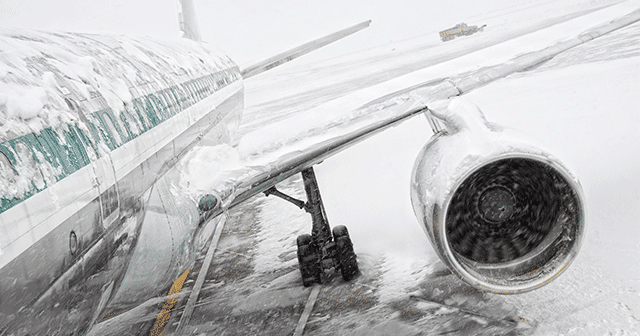
\includegraphics[width=\textwidth]{figures/wx_airplane-covered-in-ice_img-blog_0221-4139597602.png} \\
            \small{Experimental variability}
        \end{column}
    \end{columns}
\end{frame}

\begin{frame}{The Core Issue: Model Discrepancy}
    \begin{itemize}
        \item Today's numerical tools (like CFD codes for icing) lean heavily on empirical correlations and big simplifications.
        \item Because of this, we see a massive \textbf{discrepancy} between what the computer predicts and what happens in real life.
        \item Relying on just a single deterministic prediction is asking for trouble.
    \end{itemize}
    \vspace{0.5cm}
    \centering
    % 
\includegraphics[width=0.6\textwidth]{figures/intro/many_shapes_2.png} \\
    \small{Numerical variability across different icing codes~\cite{many_ice_shapes_summary}}
\end{frame}

\begin{frame}{Key Bottlenecks in Uncertainty Quantification (UQ)}
    To enable reliable virtual certification, we must address two primary UQ bottlenecks:
    \vspace{0.5cm}
    \begin{enumerate}
        \item \textbf{Model Error (Calibration):} How to rigorously identify, quantify, and treat the structural discrepancy between mathematical equations and physical phenomena without incurring prohibitive computational costs?
        \vspace{0.3cm}
        \item \textbf{Discontinuous Responses (Emulation):} How to build cheap-to-evaluate surrogate models that can accurately capture abrupt physical transitions without prior expert knowledge?
    \end{enumerate}
\end{frame}

\begin{frame}{Goal of the Thesis \& Outline}
    \begin{block}{Primary Objective}
        Advance the core methodologies of Uncertainty Quantification (UQ) to unlock practical, reliable virtual certification for complex, mis-specified, and non-smooth engineering applications.
    \end{block}
    \vspace{0.5cm}
    \textbf{Outline:}
    \begin{itemize}
        \item \textbf{Part I:} Bayesian Calibration under Model Discrepancy
        \item \textbf{Part II:} Emulation of Discontinuous Responses
        \item \textbf{Conclusions}
    \end{itemize}
\end{frame}

\section{Methodological Challenges}

\begin{frame}{Aleatoric vs Epistemic Uncertainty}
    \begin{columns}
        \begin{column}{0.5\textwidth}
            
                \textbf{Aleatoric (Irreducible)}
                \begin{itemize}
                    \item Inherent variability in the physical system.
                    \item Example: Atmospheric temperature, droplet size distribution.
                    \item Must be propagated through models.
                \end{itemize}
        \end{column}
        \begin{column}{0.5\textwidth}
            
                \textbf{Epistemic (Reducible)}
                \begin{itemize}
                    \item Lack of knowledge about the system or parameters $\btheta$.
                    \item Example: Thermal conductivity, surface roughness.
                    \item Can be reduced via \textit{inference} by combining models with data $\data$.
                \end{itemize}
        \end{column}
    \end{columns}
    \vspace{0.5cm}
    \begin{block}{Bayesian Inference}
        Treats unknown parameters as random variables:
        $$ \p{\btheta \mid \data} \propto \p{\data \mid \btheta} \prior{\btheta} $$
    \end{block}
\end{frame}

\begin{frame}{The Challenge of Model Error}
    \begin{itemize}
        \item What if the physical equations are inherently flawed?
        \item The \textit{true} value of a parameter becomes ill-defined.
        \item \textbf{Objective:} Find a suitable pair of parameters $\btheta$ and model error $\bpsi$ that best explains the data.
    \end{itemize}
    \vspace{0.3cm}
    \begin{center}
        \begin{tikzpicture}
            \node[draw, rounded corners, fill=blue!10, text width=3cm, align=center] (fb) {Full Bayesian (FB) \\ Joint Inference};
            \node[draw, rounded corners, fill=red!10, text width=3cm, align=center, right=2cm of fb] (mod) {Modular \\ Sequential Inference};
            
            \draw[->, thick] (fb) -- node[above] {Curse of dimensionality} (mod);
            \node[below=0.2cm of fb, text width=3cm, align=center, font=\small] {Coherent but intractable};
            \node[below=0.2cm of mod, text width=3cm, align=center, font=\small] {Tractable but biased (False certitude)};
        \end{tikzpicture}
    \end{center}
\end{frame}

\begin{frame}{Emulation Challenges}
    \begin{itemize}
        \item Rigorous UQ requires millions of model evaluations, demanding cheap-to-evaluate \textbf{surrogate models}.
        \item \textbf{The specific issue:} Discontinuous responses (e.g., regime shifts in icing).
    \end{itemize}
    \vspace{0.3cm}
    \begin{block}{Failure of Standard Surrogates}
        \begin{itemize}
            \item Global models (like GPs or PCEs) assume smoothness.
            \item Result: Gibbs phenomenon (spurious oscillations) near discontinuities.
            \item Biased parameters and poor convergence rates.
        \end{itemize}
    \end{block}
\end{frame}

\section[CMP Method]{The CMP Method}

\begin{frame}{Bayesian Calibration of Mis-Specified Models}
    \begin{center}
        \Large \textbf{The Complete Maximum a Posteriori (CMP) Method} \\[0.5cm]
        \normalsize How can we overcome the curse of dimensionality while preserving the rigor of a Full Bayesian analysis?
    \end{center}
\end{frame}

\begin{frame}{The Full Bayesian (FB) Formulation}
    In a Full Bayesian approach, we try to estimate the physical parameters $\btheta$ and the model error hyperparameters $\bpsi$ at the same time:
    \begin{equation*}
        \p{\btheta, \bpsi \mid \data} \propto \likelihood{\data \mid \btheta, \bpsi} \prior{\btheta} \prior{\bpsi}
    \end{equation*}
    To find what we actually care about (the physical parameters), we have to integrate out the hyperparameters:
    \begin{equation*}
        \p{\btheta \mid \data} = \intpsi{\p{\btheta, \bpsi \mid \data}}
    \end{equation*}
    
    \vspace{0.3cm}
    \textbf{The catch?} This integration is computationally prohibitive in high dimensions. It simply takes too long.
\end{frame}

\begin{frame}{The Modular Approach (KOH) and its Limitations}
    To avoid this bottleneck, the classic Kennedy and O'Hagan (KOH) approach suggests estimating the hyperparameters independently first:
    \begin{equation*}
        \psikoh = \argmax_{\bpsi} \intt{\p{\btheta, \bpsi \mid \data}}
    \end{equation*}
    Then, we just plug that estimate back in to find our parameters:
    \begin{equation*}
        \p{\btheta \mid \data, \psikoh} \propto \likelihood{\data \mid \btheta, \psikoh} \prior{\btheta}
    \end{equation*}
    
    \vspace{0.3cm}
    \textbf{The problem?} By completely ignoring the uncertainty in $\bpsi$, we end up with \textit{false certitude}—our parameter estimates look much more confident than they actually are, which can introduce dangerous bias.
\end{frame}

\begin{frame}{Introducing the Complete Maximum a Posteriori (CMP) Method}
    So, how do we fix this? Enter the Complete Maximum a Posteriori (CMP) Method.
    \vspace{0.3cm}
    
    The goal is straightforward: keep the computational efficiency of modular approaches, but perfectly match the exact Full Bayesian posterior. Instead of relying on a single, fixed $\psikoh$, we define a flexible functional mapping:
    \begin{equation*}
        \psimap = \argmax_{\bpsi \in \Psi} \p{\btheta, \bpsi \mid \data}
    \end{equation*}
    
    This couples $\bpsi$ back to $\btheta$, letting us evaluate the joint posterior along a parameter-dependent curve $\left(\btheta, \psimap\right)$.
\end{frame}

\begin{frame}{Functional Mapping: Decoupling with Coherence}
    If we break down the joint posterior using the marginal probability rule, we get:
    \begin{equation*}
        \p{\btheta, \bpsi \mid \data} = \p{\btheta \mid \data} \p{\bpsi \mid \btheta, \data}
    \end{equation*}
    
    \vspace{0.5cm}
    By looking at this, we realize that evaluating the conditional distribution $\p{\bpsi \mid \btheta, \data}$ right at its peak ($\psimap$) gives us a clever shortcut. It provides a direct pathway to marginalize the joint distribution without ever having to actually compute the difficult integral.
\end{frame}

\begin{frame}{Hessian-Based Correction Factor}
    Assuming the shape of the conditional distribution changes only by shifting and scaling:
    \begin{equation*}
        \bphi = \Stheta (\bpsi - \psimap)
    \end{equation*}
    We introduce a crucial Hessian-based correction factor $\detf{\Stheta}$ to the CMP posterior to keep everything mathematically sound:
    \begin{equation*}
        \p{\btheta \mid \data} \approx \p{\btheta, \psimap \mid \data} \dfrac{1}{\detf{\Stheta}}
    \end{equation*}
    
    \vspace{0.3cm}
    \begin{center}
        \begin{tikzpicture}[node distance=1.5cm, auto, thick, >={Stealth}]
            \node[draw, rounded corners, fill=blue!10] (map) {Compute $\psimap$};
            \node[draw, rounded corners, fill=red!10, right=of map] (hess) {Evaluate $\detf{\Stheta} \propto \sqrt{\detf{\hessian{\bpsi}}}$};
            \node[draw, rounded corners, fill=green!10, right=of hess] (post) {Corrected $\p{\btheta \mid \data}$};
            
            \draw[->] (map) -- (hess);
            \draw[->] (hess) -- (post);
        \end{tikzpicture}
    \end{center}
\end{frame}

\begin{frame}{Analytical Equivalence to Full Bayesian}
    Does this actually work? We start with a \textbf{Closed-Form Example: Well-Specified Model}.
    \vspace{0.3cm}
    
    Here, there is no structural model error, only experimental noise ($\sigma_e$).
    \begin{itemize}
        \item In this closed-form scenario, CMP perfectly matches the exact Full Bayesian marginal posterior.
        \item Traditional modular approaches suffer from \textbf{false certitude}, overemphasizing areas with small residuals and completely failing to capture the heavier tails of the true distribution.
        \item The Hessian correction factor $\detf{\Stheta}$ is what theoretically guarantees CMP's accuracy here.
    \end{itemize}
\end{frame}

\begin{frame}{Closed-Form Example: Mixture of Gaussians}
    What happens if the posterior is highly multimodal? We tested CMP on a theoretical Mixture of Gaussians.
    \vspace{0.3cm}
    
    \begin{columns}
        \begin{column}{0.5\textwidth}
            \centering
            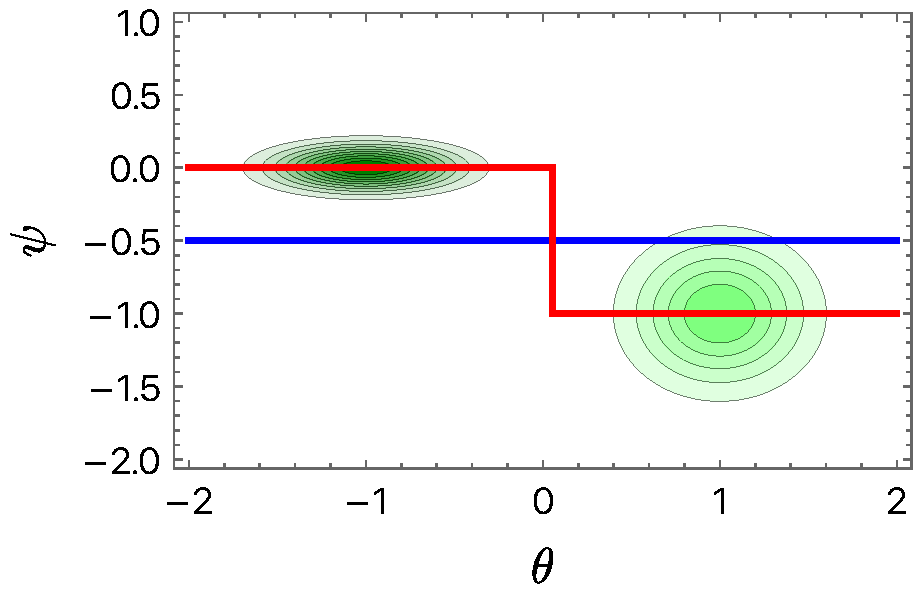
\includegraphics[width=0.9\textwidth,height=0.45\textheight,keepaspectratio]{../figures/cmp/fig_3.pdf}
            \\[0.1cm]
            \footnotesize Joint distribution with the $\psimap$ curve (red).
        \end{column}
        \begin{column}{0.5\textwidth}
            \centering
            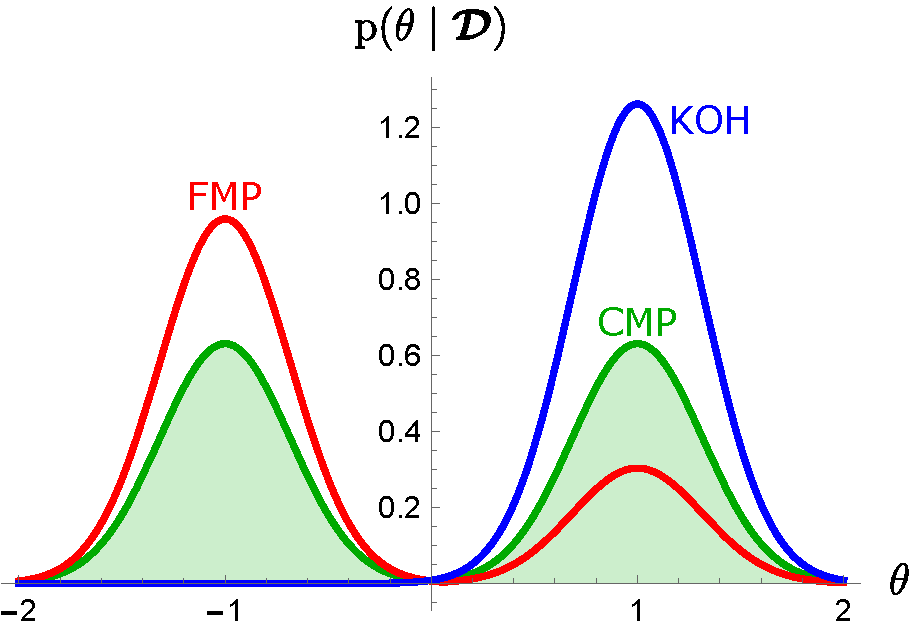
\includegraphics[width=0.9\textwidth,height=0.45\textheight,keepaspectratio]{../figures/cmp/fig_4.pdf}
            \\[0.1cm]
            \footnotesize CMP posterior matches exactly.
        \end{column}
    \end{columns}
    \vspace{0.3cm}
    CMP exactly recovers the modes and their true weights, whereas KOH collapses to a single mode.
\end{frame}

\begin{frame}{Numerical Example: Higher Dimensional Unimodal Distribution}
    We then tested CMP on a complex numerical problem with an inadequate forward model and a Gaussian Process model error term.
    
    \begin{columns}
        \begin{column}{0.5\textwidth}
            \centering
            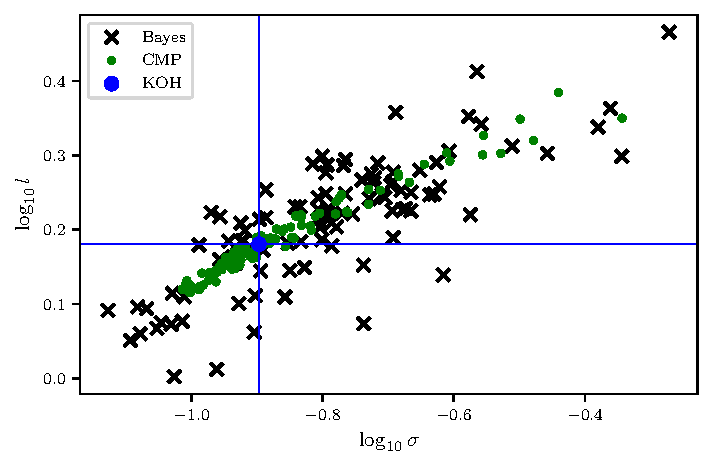
\includegraphics[width=\textwidth,height=0.5\textheight,keepaspectratio]{../figures/cmp/fig_9.pdf}
            \\[0.1cm]
            \footnotesize Joint plot of GP hyperparameters with $\psimap$.
        \end{column}
        \begin{column}{0.5\textwidth}
            \centering
            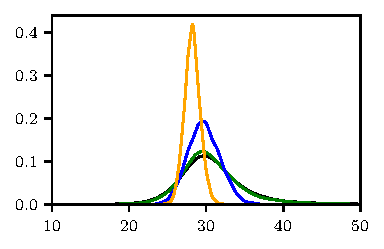
\includegraphics[width=\textwidth,height=0.5\textheight,keepaspectratio]{../figures/cmp/fig_8a.pdf}
            \\[0.1cm]
            \footnotesize Marginal posterior (CMP in green).
        \end{column}
    \end{columns}
    
    \vspace{0.3cm}
    Once again, CMP seamlessly captures the exact variance of the Full Bayesian method, avoiding the catastrophic overconfidence of KOH.
\end{frame}

\begin{frame}{Key Takeaway}
    \begin{block}{The Complete Maximum a Posteriori (CMP) Method}
        It successfully reduces a computationally expensive high-dimensional Full Bayesian problem into decoupled optimization steps. By using the Hessian correction, it explicitly prevents the False Certitude effect while maintaining scalability.
    \end{block}
\end{frame}

\section{Adaptive Sampling for CMP (AS-hGP)}

\begin{frame}{Accelerating CMP: The Computational Bottleneck}
    \begin{itemize}
        \item The CMP framework provides a robust posterior, but requires solving an optimization problem for the hyperparameters $\hat{\bpsi}_{\btheta}$ at each evaluation of $\btheta$.
        \item \textbf{Solution:} Replace the expensive mapping $\btheta \mapsto \hat{\bpsi}_{\btheta}$ with a surrogate model.
        \item \textbf{Hyperparameter Gaussian Processes (hGP):} Train a GP to predict $\hat{\bpsi}_{\btheta}$ across the parameter space.
        \item \textbf{Challenge:} Where to place the training points? We want to sample where the posterior is high, but the posterior is unknown a priori. Traditional one-shot sampling (e.g., LHS) is inefficient.
    \end{itemize}
\end{frame}

\begin{frame}{The AS-hGP Algorithm}
    AS-hGP iteratively builds the surrogate model by adaptively sampling from the posterior:
    \vspace{0.3cm}
    \begin{center}
    \begin{tikzpicture}[
        scale=0.8, transform shape,
        node distance=1.0cm and 1.5cm,
        block/.style={rectangle, draw=blue!80, thick, rounded corners, fill=blue!5, text width=4.5cm, text centered, minimum height=1.8cm, font=\small},
        arrow/.style={-{Stealth[scale=1.2]}, thick, draw=black!70},
        cond/.style={font=\footnotesize\itshape, fill=white, inner sep=2pt}
    ]

    % Nodes
    \node[block] (step1) {\textbf{Step 1: Build Surrogate}\\[1ex] $\tilde{\bpsi}(\btheta) \sim \mathcal{GP}$};
    \node[block, right=of step1] (step2) {\textbf{Step 2: Candidate Sampling}\\[1ex] $\btheta_c \sim \pi_{\text{avg}}(\btheta \mid \data)$};
    \node[block, below=of step2] (step3) {\textbf{Step 3: EVR Resampling}\\[1ex] $w_{\mathrm{res}}(\btheta) \propto \mathbb{V}_{\boldsymbol{\omega}} \left[ \phi(\btheta \mid \tilde{\bpsi}^{(\boldsymbol{\omega})})\right]$};
    \node[block, left=of step3] (step4) {\textbf{Step 4: Update}\\[1ex] $\boldsymbol{\Psi}^{(t+1)} = \boldsymbol{\Psi}^{(t)} \cup \{\text{new points}\}$};

    % Initialization and Exit
    \node[above=1cm of step1, align=center, font=\small] (init) {Initial Training Set $\boldsymbol{\Psi}^{(0)}$};
    \node[left=1.5cm of step4, align=center, font=\small] (end) {Final Surrogate\\ $\tilde{\boldsymbol{\psi}}^{(\star)}(\boldsymbol{\theta})$};

    % Arrows
    \draw[arrow] (init) -- (step1);
    \draw[arrow] (step1) -- (step2);
    \draw[arrow] (step2) -- (step3);
    \draw[arrow] (step3) -- (step4);
    \draw[arrow] (step4) -- node[right, cond] {not converged} (step1);
    \draw[arrow] (step4) -- node[above, cond] {converged} (end);

    \end{tikzpicture}
    \end{center}
\end{frame}

\begin{frame}{AS-hGP: Candidate Sampling}
    \begin{block}{Posterior-Informed Candidate Sampling}
        Candidate points are sampled from an averaged posterior over multiple GP realizations to prevent overfitting to the predictive mean.
    \end{block}
\end{frame}

\begin{frame}{AS-hGP: Variance-Based Weighted Resampling}
    \begin{block}{Variance-Based Weighted Resampling}
        Candidates are resampled using weights proportional to the variance of the potential:
        \begin{equation*}
            w_{\mathrm{res}}(\btheta_i) \propto \mathbb{V}_{\boldsymbol{\omega}} \left[ \phi(\btheta_i \mid \tilde{\bpsi}^{(\boldsymbol{\omega})}(\btheta_i))\right]
        \end{equation*}
        \begin{itemize}
            \item \textbf{Exploitation:} Candidates are already in high-probability regions.
            \item \textbf{Exploration:} Weights favor regions with high surrogate uncertainty.
            \item \textbf{Efficiency:} Rank-1 updates to the covariance inverse prevent selecting clustered points.
        \end{itemize}
    \end{block}
\end{frame}

\begin{frame}{Application: Design Under Uncertainty}
    \begin{itemize}
        \item We motivate AS-hGP using a \textbf{Design Under Uncertainty} problem.
        \item \textbf{Goal:} Predict the horizontal displacement of a planar frame.
        \item \textbf{Uncertainty:} The material (Young's modulus) is unknown and calibrated from a separate cantilever beam experiment. Unmodeled material nonlinearities act as model error.
    \end{itemize}
    \begin{center}
        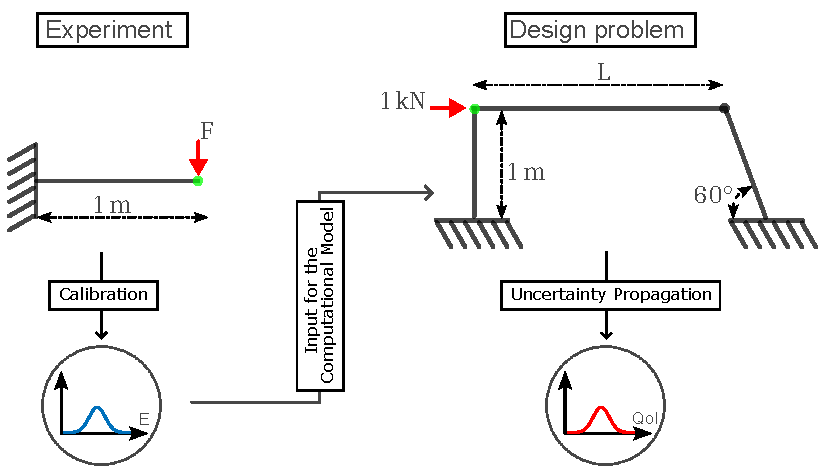
\includegraphics[width=0.9\textwidth,height=0.45\textheight,keepaspectratio]{../figures/surr/fig_4.pdf}
    \end{center}
\end{frame}

\begin{frame}{Results: Efficiency and Reliability}
    \begin{columns}
        \column{0.5\textwidth}
        \centering
        \textbf{Adaptive vs One-Shot Sampling}\\
        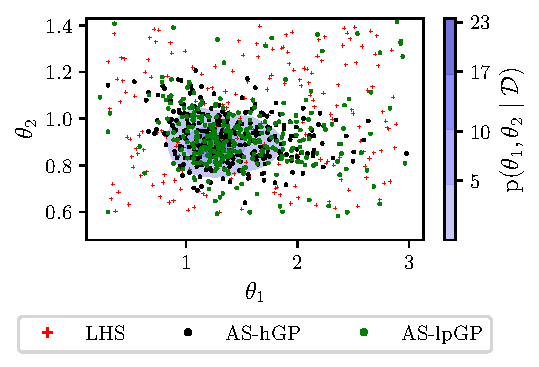
\includegraphics[width=\textwidth,height=0.6\textheight,keepaspectratio]{../figures/surr/fig_3.pdf}\\
        \footnotesize{AS-hGP concentrates training points around the true posterior (blue), unlike LHS (red).}
        
        \column{0.5\textwidth}
        \centering
        \textbf{Design Problem Prediction}\\
        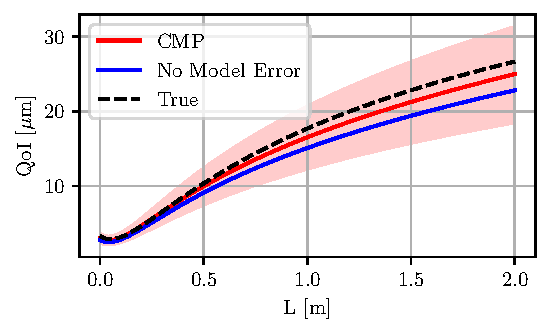
\includegraphics[width=\textwidth,height=0.6\textheight,keepaspectratio]{../figures/surr/fig_8.pdf}\\
        \footnotesize{Propagated AS-hGP posterior captures the true frame displacement reliably.}
    \end{columns}
\end{frame}

\section[Hypersonic Application]{Real-World Application: Hypersonic Flow Characterization}

\begin{frame}{VKI Plasmatron Experimental Setup}
    \begin{columns}
        \begin{column}{0.5\textwidth}
            \textbf{Our Goal}: Reconstruct catalytic efficiencies of reusable Thermal Protection Materials (TPMs) for hypersonic re-entry.
            
            \vspace{0.3cm}
            \begin{itemize}
                \item \textbf{Facility}: The VKI inductively-coupled-plasma wind tunnel.
                \item \textbf{Measurements}: We monitor the stagnation heat-flux ($q_w$) and stagnation pressure.
            \end{itemize}
        \end{column}
        \begin{column}{0.5\textwidth}
            \centering
            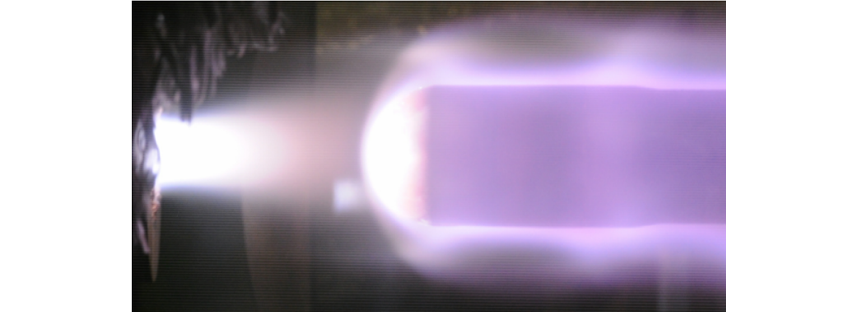
\includegraphics[width=\textwidth]{../figures/cfd/SupersonicJet.pdf}
            \\[0.2cm]
            \footnotesize Supersonic under-expanded air jet testing a TPM sample.
        \end{column}
    \end{columns}
\end{frame}

\begin{frame}{Formulating the Calibration Problem}
    Here is the catch: the total temperature $\mathrm{T}_0$ is \textit{unknown} and we can't measure it directly in the facility. 
    
    \vspace{0.3cm}
    So, we have to infer it alongside the catalytic efficiencies! Our calibration setup looks like this:
    \begin{equation*}
        \left.
        \begin{aligned}
            &q_\mathrm{w} = \tilde{q}_\mathrm{w}(\mathbf{p}; \gamma_{\mathrm{N}}, \mathrm{T}_0) + z_{q_\mathrm{w}} + \epsilon_{q_\mathrm{w}} \\
            &\mathrm{P}_\mathrm{w} = \hat{\mathrm{P}}_\mathrm{w}(\mathbf{p}; \gamma_{\mathrm{N}}, \mathrm{T}_0) + z_{\mathrm{P}_\mathrm{w}} + \epsilon_{\mathrm{P}_\mathrm{w}} \\
            &\dot{m} = \hat{m}(\mathbf{p}; \gamma_{\mathrm{N}}, \mathrm{T}_0) + z_{\dot{m}} + \epsilon_{\dot{m}} 
        \end{aligned}
        \right.
    \end{equation*}
    where $\mathbf{p}$ are our known pressure control variables.
\end{frame}

\begin{frame}{Two Types of Model Error}
    To rigorously test our framework, we deliberately introduce realistic model error by employing two different solvers:
    \vspace{0.3cm}
    \begin{columns}
        \begin{column}{0.5\textwidth}
            \begin{itemize}
                \item \textbf{Experimental Bias}: We introduce an artificial bias to the heat-flux measurements to emulate un-modeled facility effects.
                \item \textbf{Model Discrepancy}: We compare predictions from a high-fidelity 3D \texttt{US3D} solver against a heavily simplified quasi-1D \texttt{STAGLINE} solver.
            \end{itemize}
        \end{column}
        \begin{column}{0.5\textwidth}
            \centering
            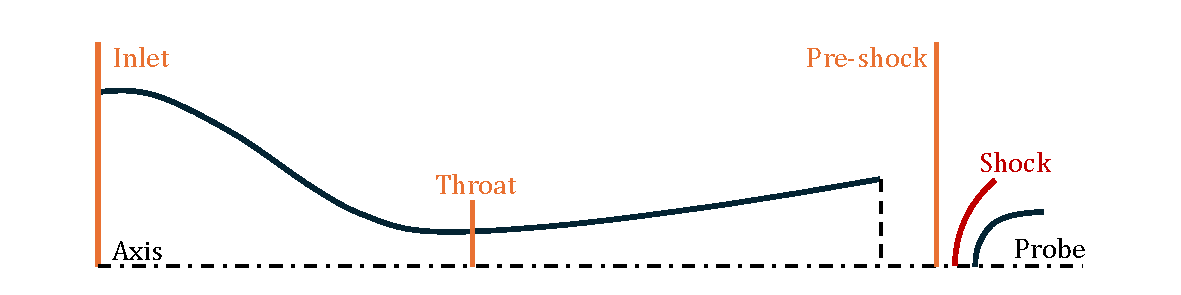
\includegraphics[width=0.9\textwidth,height=0.4\textheight,keepaspectratio]{../figures/cfd/LowFidelity.pdf}
        \end{column}
    \end{columns}
    \vspace{0.3cm}
    \textit{The fundamental discrepancy mimics the kind of severe, real-world model inadequacy that causes traditional calibration methods to fail.}
\end{frame}

\begin{frame}{Results: Reconstructing Catalytic Efficiencies}
    We calibrate the models using the KOH and Full Bayesian (FB) methods to rigorously evaluate the impact of these two model error types.
    
    \vspace{0.3cm}
    \begin{itemize}
        \item \textbf{Key Finding 1}: Ignoring model error (using standard Bayesian inversion) leads to severe bias and overconfidence; the inferred catalytic efficiencies absorb the un-modeled physics.
        \item \textbf{Key Finding 2}: Incorporating a proper model error term correctly inflates the uncertainty bounds, preventing dangerous false certitude in the design of thermal protection systems.
    \end{itemize}
\end{frame}

\section[Clustering]{Piecewise Emulation via Clustering \& Classification}

\providecommand{\bbeta}{\boldsymbol{\beta}}
\providecommand{\bgamma}{\boldsymbol{\gamma}}
\providecommand{\Sglobal}{S_{\mathrm{global}}}

\begin{frame}{Standard Surrogates Near Discontinuities}
    \begin{columns}[c]
        \begin{column}{0.5\textwidth}
            \begin{itemize}
                \item Standard GPs and PCEs assume global smoothness.
                \item Spectral methods suffer from the Gibbs phenomenon (oscillations near the jump).
                \item GPs smear boundaries \& artificially inflate uncertainty everywhere.
                \item Result: A surrogate model we cannot fully trust for virtual certification.
            \end{itemize}
        \end{column}
        \begin{column}{0.5\textwidth}
            \centering
            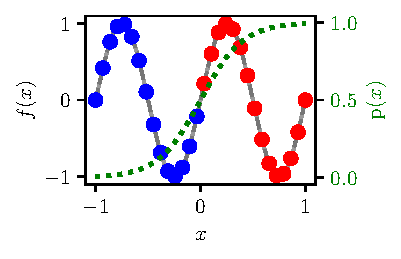
\includegraphics[width=0.9\textwidth,height=0.4\textheight,keepaspectratio]{../figures/sota_2/gp_realizations_demo.pdf}
        \end{column}
    \end{columns}
\end{frame}

\begin{frame}{The Need for a Problem-Independent Approach}
    \begin{itemize}
        \item Complex simulations (e.g., in-flight icing) feature abrupt regime transitions without explicit flags.
        \item Prior expert knowledge to manually partition the input space ($\bx$) is rarely available.
        \item We need a \textbf{data-driven learning} strategy to discover discontinuities automatically.
        \item Goal: Cluster data, train local models, and define boundaries with \textbf{no manual hand-holding}.
    \end{itemize}
\end{frame}

\begin{frame}{Proposed Methodology: Iterative Coupling}
    \begin{block}{Piecewise Surrogate Model Formulation}
        We can think of our surrogate as a patchwork of simpler, local models glued together by a classifier:
        \begin{equation}
            \tilde{f}(\bx; \bbeta, \mathcal{P}) = \sum_{l=1}^L \mathbb{I}_{\Omega_l}(\bx; \bgamma) \tilde{f}_l(\bx; \bbeta_l)
        \end{equation}
    \end{block}
    \vspace{0.2cm}
    \begin{itemize}
        \item $\bz$: Tells us which data points belong to which cluster.
        \item $\mathbb{I}_{\Omega_l}(\bx; \bgamma)$: The classifier that draws the boundaries between regions.
        \item $\tilde{f}_l(\bx; \bbeta_l)$: Our localized experts (the regressors).
        \item \textbf{The hard part:} We have to jointly optimize the memberships, boundaries, and model parameters without getting trapped in bad local minima.
    \end{itemize}
\end{frame}

\begin{frame}{The Algorithmic Loop}
    \centering
    \vspace{0.3cm}
    \begin{tikzpicture}[
        node distance=1cm and 1.5cm,
        block/.style={rectangle, draw=black, fill=blue!10, text width=2.8cm, text centered, rounded corners, minimum height=1.2cm, thick},
        arrow/.style={-{Stealth[scale=1.2]}, thick}
    ]
        % Nodes
        \node[block] (clust) {1. Propose New\\ $\bz^{(t+1)}$};
        
        \node[block, right=of clust] (regress) {2. Update Local\\ $\bbeta^{(t+1)}$};
        \draw[arrow] (clust) -- (regress);
        
        \node[block, below=of regress] (class) {3. Update Classifier\\ $\bgamma^{(t+1)}$};
        \draw[arrow] (regress) -- (class);
        
        \node[block, left=of class] (score) {4. Evaluate Global\\ Score $\Sglobal$};
        \draw[arrow] (class) -- (score);
        \draw[arrow] (score) -- (clust);
    \end{tikzpicture}
    
    \vspace{0.5cm}
    \begin{itemize}
        \item Instead of solving everything at once, we use an iterative approach.
        \item We start with a rough guess and let the local models dictate how to improve the clusters.
        \item Because the loop is modular, you can plug in whatever regressor or classifier you prefer.
    \end{itemize}
\end{frame}

\begin{frame}{Model-Based Clustering \& Global Score}
    \begin{block}{Global Score Function $\Sglobal$}
        We measure how good our patchwork model is by summing up the local scores (like log-marginal likelihoods):
        \begin{equation}
            \Sglobal(\bbeta, \bz) = \sum_{l=1}^L S(\bbeta_l, \data_l(\bz))
        \end{equation}
    \end{block}
    
    \begin{itemize}
        \item By keeping the score local, we can actually train all our regressors in parallel.
        \item We decide whether to move a point to a new cluster by checking if it improves this overall score ($\Delta S$).
        \item But there's a catch: if we just greedily maximize the score, the algorithm might create tiny, meaningless clusters just to fit the noise perfectly.
    \end{itemize}
\end{frame}

\begin{frame}{Stochastic Membership Updates \& Convergence}
    To stop the model from overfitting, we introduce some randomness controlled by a "temperature" parameter:
    
    \begin{equation}
        \mathbb{P}(l \rightarrow l^{\prime}) \propto \exp \left( \frac{1}{T} \Delta S \right) \, h\left(\mathbb{P}_{\mathrm{CLS}}(l^\prime \mid \bx, \bgamma) \right)
    \end{equation}

    \begin{itemize}
        \item \textbf{Exploration (High $T$):} When things are "hot", the classifier's uncertainty drives the bus. Points can freely jump across boundaries to explore new setups.
        \item \textbf{Exploitation ($T \rightarrow 0$):} As we cool things down, the model becomes greedy, locking into the best score.
    \end{itemize}
    
    \begin{block}{Convergence Properties}
        From a mathematical standpoint, this cooling process guarantees that we eventually settle on a stable, optimal partition (or enter a mild, easily detectable limit cycle).
    \end{block}
\end{frame}

\begin{frame}{The Evolution of Model-Based Clustering}
    \begin{center}
        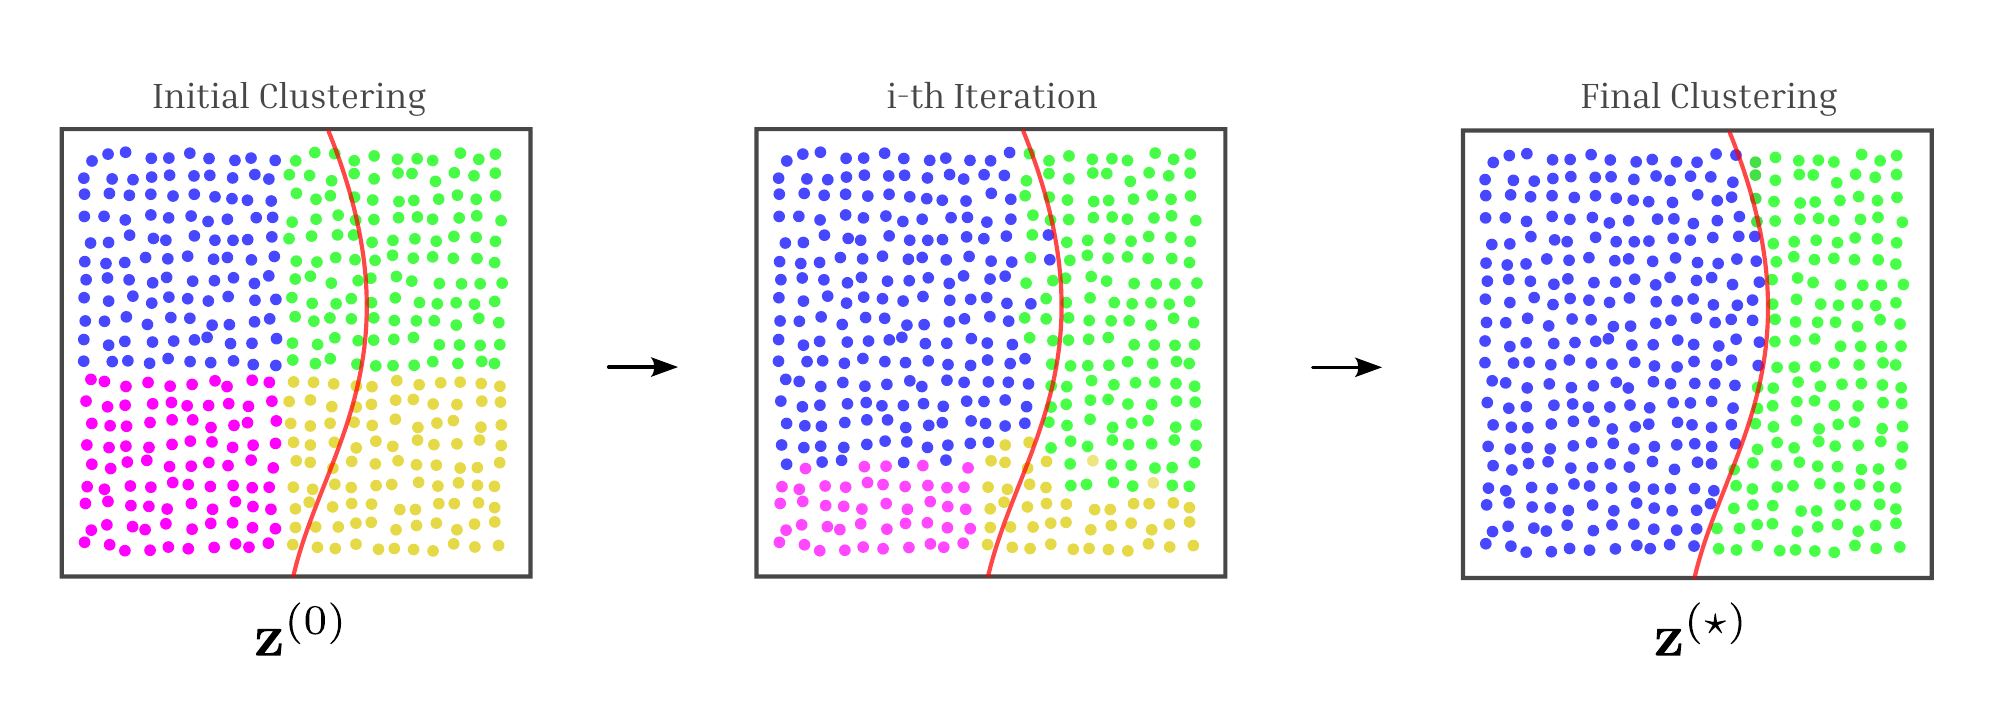
\includegraphics[width=0.85\textwidth,height=0.6\textheight,keepaspectratio]{../figures/clustering/Evolution.png}
    \end{center}
    \vspace{0.2cm}
    \begin{itemize}
        \item The algorithm iteratively discovers both the boundaries (classifier) and the smooth physical regimes (regressors) simultaneously.
    \end{itemize}
\end{frame}

\begin{frame}{Numerical Example 1: 1D Jump}
    \begin{columns}[c]
        \begin{column}{0.4\textwidth}
            \begin{itemize}
                \item Let's look at a simple 1D function with a sharp jump.
                \item A naive clustering (e.g., K-Means or single GP) gets it completely wrong by trying to smooth across the jump.
                \item The proposed algorithm neatly pinpoints the exact location of the jump, recovering a \textbf{good clustering} without Gibbs oscillations.
            \end{itemize}
        \end{column}
        \begin{column}{0.6\textwidth}
            \centering
            Naive approach:\\
            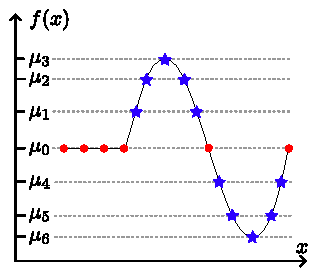
\includegraphics[width=0.8\textwidth,height=0.35\textheight,keepaspectratio]{../figures/clustering/badClustering.pdf}\\
            Our approach:\\
            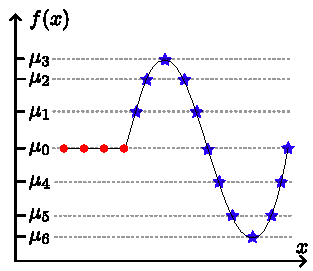
\includegraphics[width=0.8\textwidth,height=0.35\textheight,keepaspectratio]{../figures/clustering/goodClustering.pdf}
        \end{column}
    \end{columns}
\end{frame}

\begin{frame}{Numerical Example 2: Higher Dimensions}
    \begin{columns}[c]
        \begin{column}{0.5\textwidth}
            \begin{itemize}
                \item In higher dimensions, the boundaries between physical regimes can take on complex, non-convex shapes.
                \item Thanks to the stochastic annealing, the algorithm doesn't easily get trapped in bad local configurations.
                \item By pairing it with a strong classifier, we can trace out highly irregular boundaries effortlessly.
                \item It neatly separates the data without us ever having to label the physics manually.
            \end{itemize}
        \end{column}
        \begin{column}{0.5\textwidth}
            \centering
            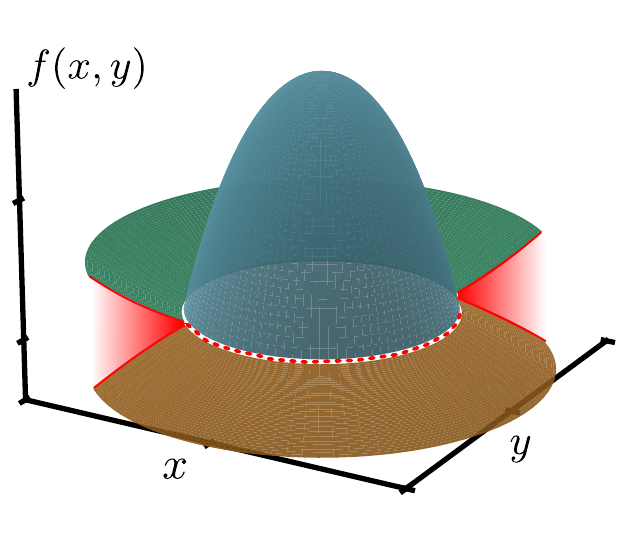
\includegraphics[width=0.9\textwidth,height=0.35\textheight,keepaspectratio]{../figures/clustering/function_plot_compressed.png}\\
            \vspace{0.2cm}
            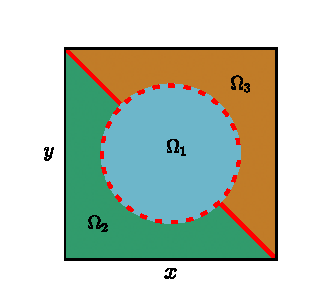
\includegraphics[width=0.9\textwidth,height=0.35\textheight,keepaspectratio]{../figures/clustering/partition_plot.pdf}
        \end{column}
    \end{columns}
\end{frame}

\begin{frame}{Taming Over-Clustering}
    \begin{columns}[c]
        \begin{column}{0.5\textwidth}
            \begin{itemize}
                \item \textbf{Risk:} Over-segmenting perfectly smooth domains.
                \item \textbf{Solution:} Merge adjacent clusters using a classifier "confusion metric".
                \item \textbf{Result:} A highly robust, hands-off workflow for handling tricky physics.
            \end{itemize}
        \end{column}
        \begin{column}{0.5\textwidth}
            \centering
            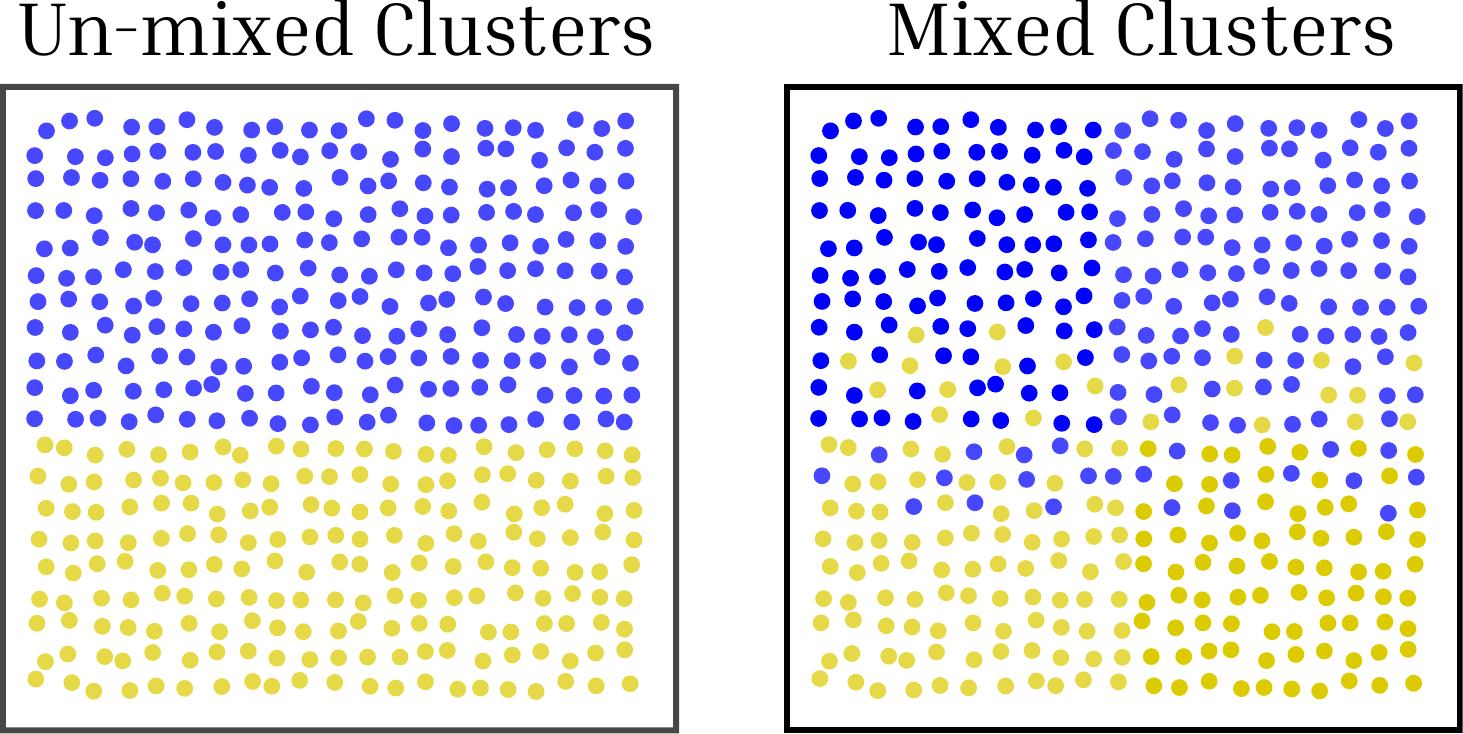
\includegraphics[width=0.9\textwidth]{../figures/clustering/confusion.png}
        \end{column}
    \end{columns}
\end{frame}

\section[Conclusion]{Conclusion \& Future Work}

\begin{frame}{Summary of Part I}
    \begin{block}{CMP \& Surrogate Acceleration}
        \begin{itemize}
            \item \textbf{Bridging the Gap:} CMP unifies Full Bayesian exactness with Modular calibration speed.
            \item \textbf{No False Certitude:} Decouples hyperparameter optimization while preserving Full Bayesian bounds.
            \item \textbf{Acceleration (AS-hGP):} Expected Variance Reduction drastically speeds up inference.
            \item \textbf{Validation:} Successfully resolved missing data and severe model error in hypersonic flows.
        \end{itemize}
    \end{block}
\end{frame}

\begin{frame}{Summary of Part II}
    \begin{block}{Piecewise Emulation of Discontinuous Responses}
        \begin{itemize}
            \item \textbf{Data-Driven Discovery:} Emulates discontinuous physics without prior expert knowledge.
            \item \textbf{Iterative Coupling:} Unifies clustering, classification, and regression into a robust loop.
            \item \textbf{Overcoming Limitations:} Successfully eliminates Gibbs oscillations and global regressor smearing.
        \end{itemize}
    \end{block}
\end{frame}

\begin{frame}{Future Perspectives}
    \begin{itemize}
        \item \textbf{Active Learning for Piecewise Surrogates:} Extend the Expected Variance Reduction criterion (ALC) to efficiently train the clustering-based surrogate model (non-Gaussian mixture).
        \item \textbf{Integration:} Directly couple the piecewise emulator within the calibration loop to enable robust inference for discontinuous physics (e.g., icing regime shifts).
    \end{itemize}
    \vspace{0.5cm}
    \begin{center}
        \begin{tikzpicture}
            \node[draw, rounded corners, fill=green!10, text width=4cm, align=center] (uq) {Robust UQ \& Calibration};
            \node[draw, rounded corners, fill=orange!10, text width=4cm, align=center, right=1.5cm of uq] (surr) {Piecewise Emulation};
            
            \draw[<->, thick, shorten >=2pt, shorten <=2pt] (uq) -- (surr);
            \node[below=0.2cm of uq, text width=4cm, align=center, font=\small] {Identifies domains of interest};
            \node[below=0.2cm of surr, text width=4cm, align=center, font=\small] {Accelerates inference};
        \end{tikzpicture}
    \end{center}
\end{frame}

\begin{frame}{Impact on the Future of In-Flight Icing Research}
    \begin{itemize}
        \item Enable truly probabilistic morphogenetic models.
        \item Combine UQ techniques with similarity measures of ice shapes.
        \item Design robust anti-icing systems through global sensitivity and the Icing Severity Index (ISI).
    \end{itemize}
    \vspace{0.5cm}
    \begin{block}{Final Remark}
        The methodological advancements of this thesis provide the mathematical foundation required to transition highly complex aerospace phenomena towards a reliable, simulation-based design and virtual certification paradigm.
    \end{block}
\end{frame}




%%%%%%%%%%%%%%%%%%%%
%%%  BACKMATTER  %%%
%%%%%%%%%%%%%%%%%%%%
	\begin{frame}[noframenumbering, allowframebreaks]{References}
		\printbibliography[heading=none]
	\end{frame}

\addtocounter{levelstanda}{-1}
\end{document}
